\documentclass
[
    twoside,                 % The thesis is formatted like a book. That is, odd and even pages are handled differently.
    openright,               % Starts a new chapter on an odd page number (right side).
    cleardoublepage = empty, % Clear pages inserted in order to have new chapters appear on odd pages are formatted with an empty style.
    fontsize = 12 pt,        % The size of the font.
    british,                 % Support for British English.
    captions = tableheading, % Places the correct amount of space when the caption of a table is above the table.
    numbers = noenddot,      % Does not use a period at the end of numbered titles, such as sections or figures.
    footheight = 35 pt,      % Defines the height of the foot. Due to the line, it needs extra height.
%    draft,                   % Only displays boxes of figures. This option is useful if compilation takes a long time.
]
{scrbook}


% This file contains all sorts of commands that are used in order to specify certain options for the document.

\newif\ifprintVersion   % Defines a binary variable that signals whether the document is prepared for physical or digital print.
\newif\ifprofessionalPrint % Defines a binary variable that signals whether the print will be done by a professional printing service that requests extra margin for page cutting and is not bound to paper formats like A4.
\newif\iffancyTheorems  % Defines a binary variable that signals whether theorems are formatted in the classical style or in a new format that better suits the overall flavor of this thesis.
\newif\ifboldNumberSets % Defines a binary variable that signals whether the variables for number sets (like N or R) should be in bold. If not, they are in blackboard bold instead.
\newif\ifbachelorThesis % Defines a binary variable that signals whether this thesis is a bachelor thesis (true) or a master thesis (false).

% Set all variables to their default values.
\printVersionfalse
\professionalPrintfalse
\fancyTheoremstrue
\boldNumberSetstrue
\bachelorThesistrue

%%%%%%%%%%%%%%%%%%%%%%%%
% The following commands define certain strings that provide important information for the document.

% The title of the thesis.
\newcommand*{\printTitle}{}
\newcommand*{\printGermanTitle}{}
\newcommand*{\myTitle}[2]{\renewcommand*{\printTitle}{#1}\renewcommand*{\printGermanTitle}{#2}}
\newcommand*{\printTitleBold}{\textbf{\printTitle}}

% The author’s name.
\newcommand*{\printAuthor}{}
\newcommand*{\myName}[1]{\renewcommand*{\printAuthor}{#1}}

% The name of the author’s program.
\newcommand*{\printProgram}{}
\newcommand*{\myProgram}[1]{\renewcommand*{\printProgram}{#1}}

% The date when the thesis was handed in.
\newcommand*{\printDateReceived}{}
\newcommand*{\dateOfHandingIn}[1]{\renewcommand*{\printDateReceived}{#1}}

% A short description of the topic of the thesis. This string will be used for the PDF metadata.
\newcommand*{\printSubject}{}
\newcommand*{\mySubject}[1]{\renewcommand*{\printSubject}{#1}}

% A short description of the topic of the thesis. This string will be used for the PDF metadata.
\newcommand*{\printKeywords}{}
\newcommand*{\myKeywords}[1]{\renewcommand*{\printKeywords}{#1}}

% The name of the author’s supervisor.
\newcommand*{\printNameOfSupervisor}{}
\newcommand*{\nameOfMySupervisor}[1]{\renewcommand*{\printNameOfSupervisor}{#1}}

% The list with the name of the additional examiners.
\newcommand*{\printAdditionalExaminers}{}
\newcommand*{\additionalExaminers}[1]{\renewcommand*{\printAdditionalExaminers}{#1}}

% Defines the extra length added to each side for the print version.
\newlength{\extraborderlength}
\newcommand*{\extraBorder}[1]{\setlength{\extraborderlength}{#1}}

% Defines the length of the binding correction. (The class ›scrbook‹ has a binding correction but it does not work due to all the other packages that are loaded.)
\newlength{\mybindingcorrection}
\newcommand*{\bindingCorrection}[1]{\setlength{\mybindingcorrection}{#1}} % Contains commands that are used for certain information that is printed.


%%%%%%%%%%%%%%%%%%%%%%%%%%%%%%%%%%%%%%
%% Please adjust your options here. %%
%%%%%%%%%%%%%%%%%%%%%%%%%%%%%%%%%%%%%%

    % This section contains commands with important data for your thesis. Please adjust them in order for the document to be printed correctly.

    % Defines the length of the amount that a printed page will be cut from EACH side (including the inner side). This option only takes effect with \printVersiontrue and \professionalPrinttrue.
    \extraBorder{3 mm}

    % Shifts the inner margin outward by the amount specified. When the book is bound, part of the page will not be seen anymore. This option compensates for this loss. It only takes effect with \printVersiontrue.
    \bindingCorrection{6 mm}

    % Use the following command if this is a master thesis.
%    \bachelorThesisfalse

%    \printVersiontrue      % Use this value if you want to prepare your thesis for physical printing. In this case, links will not be coloured. Without \professionalPrinttrue, the content will be moved outward by the binding correction, increasing the inner margin and decreasing the outer margin.
%    \professionalPrinttrue % Use this value if you want to have extra border for cutting and are not bound to paper formats (like A4). This option will increase the page size by the extra border on every side plus the binding correction once for the width. It only takes effect in combination with \printVersiontrue.
%    \fancyTheoremsfalse  % Use this value if you want to use the classical theorem style, where the text is italic. Further, with this style, the QED symbol is colourless.
%    \boldNumberSetsfalse % Use this value if you want variables for number sets (like N or R) to appear in blackboard bold rather than bold.

    % The title of the thesis. The first argument is for the English name, the second is for the German name.
    \myTitle{English Title}{Deutscher Titel}

    % The author’s name.
    \myName{Nikkel Mollenhauer}

    % The author’s program.
    \myProgram{IT-Systems Engineering}

    % The date when the thesis will be handed in.
    \dateOfHandingIn{30. Juni 2022}

    % The name and affiliation of the author’s supervisor.
    \nameOfMySupervisor{Dr. Rainer Schlosser}

    % A list with the names of the additional examiners.
    \additionalExaminers{Johannes Huegle\newline Alexander Kastius}

    % A short summary of the thesis. These information will be used for the PDF meta data.
    \mySubject{A cool bachelor thesis.}

    % Some keywords of the thesis. These information will be used for the PDF meta data. Please use | as a separator and try to avoid commas.
    \myKeywords{bachelor thesis | reinforcement learning | python | dynamic pricing | recommerce}

%%%%%%%%%%%%%%%%%%%%%%%%%%%%%%%%%%%%%%
%% End of options to adjust. %%%%%%%%%
%%%%%%%%%%%%%%%%%%%%%%%%%%%%%%%%%%%%%%


% This file includes all of the code that is used to format the thesis.
% Some packages are included if they are needed. This is done in the respective part and not at the beginning of this file.
%
% This file contains the following parts:
%   • Language an Character Set
%   • Penalties
%   • Indentation
%   • Footnotes
%   • Colors
%   • Size and Position of the Text Body
%   • Position of the Head and the Foot
%   • Margin Position and Width
%   • Header and Footer Format
%   • Caption Format
%   • Part Format
%   • Chapter Format
%   • Table of Contents


%%%%%%%%%%%%%%%%%%%%%%%%%%%%%%%%
%% Language and Character Set %%
%%%%%%%%%%%%%%%%%%%%%%%%%%%%%%%%

\usepackage[utf8]{inputenc} % Allows to input UTF8 characters.
\usepackage[T1]{fontenc}    % Allows to print special characters correctly.
\usepackage
[
    ngerman,         % German is used for the German abstract.
    main = british,  % This is the main language of the thesis.
]
{babel}                     % Is responsible for sensible hyphenations.

% The following two commands make it such that the LaTeX compiler of Overleaf produces a PDF from with ligatures and mathematical symbols can be copied correctly.
% Also refer to: https://tex.stackexchange.com/questions/64188/what-are-good-ways-to-make-pdflatex-output-copy-and-pasteable
\input glyphtounicode
\pdfgentounicode=1


%%%%%%%%%%%%%%%
%% Penalties %%
%%%%%%%%%%%%%%%

\widowpenalties 2 10000 0


%%%%%%%%%%%%%%%%%
%% Indentation %%
%%%%%%%%%%%%%%%%%

\usepackage{calc} % Makes it easer to do math with TeX measurements.

\newlength{\myparindent}
\newlength{\myparskip}
\setlength{\myparindent}{1 em}
\setlength{\myparskip}{0 em}

\setlength{\parindent}{\myparindent}
\setlength{\parskip}{\myparskip}
\setlength{\parskip}{0 pt plus 1 pt minus 0 pt}


%%%%%%%%%%%%%%%
%% Footnotes %%
%%%%%%%%%%%%%%%

% Remove the footnote rule.
\setfootnoterule{0 cm}

% The footnote number is made bold and not in superscript.
\deffootnote[1.2 em]{1.2 em}{0 em}{\makebox[1.4 em][l]{\textbf{\thefootnotemark}}}

% The footnote number will not be reset after every chapter.
\makeatletter%
    \@removefromreset{footnote}{chapter}%
\makeatother


%%%%%%%%%%%%
%% Colors %%
%%%%%%%%%%%%

\usepackage[dvipsnames]{xcolor} % Allows it to define colors. The option says that common names can be used.

% Dark blue.
\definecolor{stroke1}{HTML}{2574A9} % This color is used as the standard color to highlight things.


% Coloring various different labels.
\colorlet{captionlabel}{black}
\colorlet{footerpagenr}{black}
\colorlet{footerchapter}{stroke1}
\colorlet{footerchaptername}{black}
\colorlet{footersection}{stroke1}
\colorlet{footersectionname}{black}
\colorlet{chapternumber}{stroke1}


%%%%%%%%%%%%%%%%%%%%%%%%%%%%%%%%%%%%%%%%
%% Size and Position of the Text Body %%
%%%%%%%%%%%%%%%%%%%%%%%%%%%%%%%%%%%%%%%%

% The new paper dimensions that are exclusively used.
\newlength{\mypaperwidth}
\setlength{\mypaperwidth}{210 mm}

\newlength{\mypaperheight}
\setlength{\mypaperheight}{297 mm}

% The text area uses aesthetically pleasing measurements in the same ratio as the page.
% These dimensions are always used, as the text area should be the same in the printed and digital version of the thesis.
\newlength{\mybodywidth}
\setlength{\mybodywidth}{140 mm}

\newlength{\mybodyheight}
\setlength{\mybodyheight}{198 mm}

\newlength{\myoutermargin}
\ifprintVersion
    \ifprofessionalPrint
        \setlength{\myoutermargin}{(\mypaperwidth - \mybodywidth) / \real{1.5} + \extraborderlength}
    \else
        \setlength{\myoutermargin}{(\mypaperwidth - \mybodywidth) / \real{1.5} - \mybindingcorrection}
    \fi
\else
    \setlength{\myoutermargin}{(\mypaperwidth - \mybodywidth) / \real{1.5}}
\fi

\newlength{\mytopmargin}
\setlength{\mytopmargin}{(\mypaperheight - \mybodyheight) / 3}
\ifprintVersion
    \ifprofessionalPrint
        \setlength{\mytopmargin}{(\mypaperheight - \mybodyheight) / 3 + \extraborderlength}
    \fi
\fi

\newlength{\myinnermargin}
\setlength{\myinnermargin}{\mypaperwidth - \mybodywidth - \myoutermargin}
\ifprintVersion
    \ifprofessionalPrint
        \setlength{\myinnermargin}{\mypaperwidth + \mybindingcorrection + 2\extraborderlength - \mybodywidth - \myoutermargin}
    \fi
\fi

\newlength{\mybottommargin}
\setlength{\mybottommargin}{\mypaperheight - \mybodyheight - \mytopmargin}
\ifprintVersion
    \ifprofessionalPrint
        \setlength{\mybottommargin}{\mypaperheight + 2\extraborderlength - \mybodyheight - \mytopmargin}
    \fi
\fi


%%%%%%%%%%%%%%%%%%%%%%%%%%%%%%%%%%%
%% Position of the Head And Foot %%
%%%%%%%%%%%%%%%%%%%%%%%%%%%%%%%%%%%

\newcommand{\goldenratio}{1.618}

\newlength{\myheadsep} % Distance from the header to the body.
\setlength{\myheadsep}{\mytopmargin / \real{\goldenratio} / \real{\goldenratio} - 1 ex}
\ifprintVersion
    \ifprofessionalPrint
        \setlength{\myheadsep}{(\mytopmargin - \extraborderlength) / \real{\goldenratio} / \real{\goldenratio} - 1 ex}
    \fi
\fi

\newlength{\myfootskip} % Distance from the body to the footer.
\setlength{\myfootskip}{\mybottommargin / \real{\goldenratio} - 1 ex}
\ifprintVersion
    \ifprofessionalPrint
        \setlength{\myfootskip}{(\mybottommargin - \extraborderlength) / \real{\goldenratio} - 1 ex}
    \fi
\fi


%%%%%%%%%%%%%%%%%%%%%%%%%%%%%%%
%% Margin Position And Width %%
%%%%%%%%%%%%%%%%%%%%%%%%%%%%%%%

\newlength{\mymargininnersep} % Distance between the margin and the body.
\setlength{\mymargininnersep}{7 mm}

\newlength{\mymarginoutersep} % Distance between the margin and the paper border.
\setlength{\mymarginoutersep}{12 mm}
\ifprintVersion
    \ifprofessionalPrint
        \setlength{\mymarginoutersep}{12 mm + \extraborderlength}
    \fi
\fi

\newlength{\mymarginwidth} % Width of the margin.
\setlength{\mymarginwidth}{\myoutermargin - \mymargininnersep - \mymarginoutersep}

\newlength{\mymarginwidthwithinnersep} % Width of the margin.
\setlength{\mymarginwidthwithinnersep}{\mymarginwidth + \mymargininnersep}

\usepackage
[
    % In the printed version, we add an extra border to each side as well as the binding correction for the width.
    \ifprintVersion
        \ifprofessionalPrint
            paperwidth = \mypaperwidth + 2\extraborderlength + \mybindingcorrection,
            paperheight = \mypaperheight + 2\extraborderlength,
        \else
            paperwidth = \mypaperwidth,
            paperheight = \mypaperheight,
        \fi
    \else
        paperwidth = \mypaperwidth,
        paperheight = \mypaperheight,
    \fi
    textwidth = \mybodywidth,
    textheight = \mybodyheight,
    outer = \myoutermargin,
    top = \mytopmargin,
    headsep = \myheadsep,
    footskip = \myfootskip,
    marginparsep = \mymargininnersep,
    marginparwidth = \mymarginwidth,
%    showframe, % Use this option for debugging purposes in order to the an outline of all of the different parts of the page layout.
]
{geometry} % Used in order to define the dimensions of the page and its layout.


%%%%%%%%%%%%%%%%%%%%%%%%%%%%%%
%% Header and Footer Format %%
%%%%%%%%%%%%%%%%%%%%%%%%%%%%%%

\usepackage
[
%    draft, % Shows a lot of rules denoting the dimensions of the head and foot. Use this option only for debugging.
]
{scrlayer-scrpage} % Allows to adjust the definitions of the head and foot of a page.

%%%%%%%%%%%%%%%%%%%%%%%%%%%%%%
% Dimensions and formats are defined.

% Define the dimensions of the head and the foot. Since we want some information to appear in the margin, we extend the head and the foot by the respective lengths.
\KOMAoptions
{%
    headwidth = \textwidth + \mymarginwidthwithinnersep,%
    footwidth = \myoutermargin : \textwidth,%
}

% Defines the formats for the chapter and section titles in the marks of the head.
\renewcommand*{\chaptermarkformat}{\normalfont\sffamily\small\color{footerchaptername}}
\renewcommand*{\sectionmarkformat}{\normalfont\sffamily\small\color{footersectionname}}

% Displays the chapter names in the head of both odd and even pages.
\automark[chapter]{chapter}
% Replaces the chapter name to the head of right pages with the section name if a section is present.
\automark*[section]{}

%%%%%%%%%%%%%%%%%%%%%%%%%%%%%%
% The head is defined.

% Head for even pages.
% Puts ›Chapter‹ followed by the current chapter number.
\lehead%
{%
    \begin{minipage}[b]{\mymarginwidth}%
        \small\raggedleft\normalfont\textsf{\textbf{\color{footerchapter}\chaptername\ \thechapter}}
    \end{minipage}
}
% Put the title of the current chapter/section into the center of the head but push it to the border.
\cehead{\hspace*{\mymarginwidthwithinnersep}\parbox{\textwidth}{\raggedright\leftmark}}

% Head for odd pages.
\rohead%
{%
    % Check whether a section has already started or not.
    \Ifstr{\rightmark}{\leftmark}%
    {%
        \begin{minipage}[b]{\mymarginwidth}%
            \small\raggedright\normalfont\textsf{\textbf{\color{footersection}Chapter\ \thechapter}}%
        \end{minipage}%
    }%
    {%
        \begin{minipage}[b]{\mymarginwidth}%
            \small\raggedright\normalfont\textsf{\textbf{\color{footersection}Section\ \thesection}}%
        \end{minipage}%
    }%
}
\cohead{\hspace*{-\mymarginwidthwithinnersep}\parbox{\textwidth}{\raggedleft\rightmark}}

%%%%%%%%%%%%%%%%%%%%%%%%%%%%%%
% The foot is defined.

% Displays the page number in bold in the margin, aligned toward the center. Further, a blue line is drawn above number.
% The starred variant is used, since we want the format of the foot to also apply to the pagestyle ›plain‹.
\lefoot*%
{%
    \vspace*{1 ex}%
    {\color{stroke1}\rule{\myoutermargin - \mymargininnersep}{0.5 mm}}\\
    \begin{minipage}[b]{\myoutermargin - \mymargininnersep}%
        \raggedleft\normalfont\color{footerpagenr}\textbf{\thepage}%
    \end{minipage}%
}
\rofoot*%
{%
    {\color{stroke1}\rule{\myoutermargin - \mymargininnersep}{0.5 mm}}\\
    \begin{minipage}[b]{\myoutermargin - \mymargininnersep}%
        \raggedright\normalfont\color{footerpagenr}\textbf{\thepage}%
    \end{minipage}%
}


%%%%%%%%%%%%%%%%%%%%
%% Caption Format %%
%%%%%%%%%%%%%%%%%%%%

\usepackage{caption}
\captionsetup
{
    font = small,
    labelfont = {bf, sf, color = captionlabel},
    format = plain,
    singlelinecheck = off,
}


%%%%%%%%%%%%%%%%%
%% Part Format %%
%%%%%%%%%%%%%%%%%
\usepackage{tikz} % Used in order to draw the stylistic elements.

\newlength{\mytmpa}
\setlength{\mytmpa}{1 mm}
\newlength{\mytmpb}
\newlength{\mytmpc}

%%%%%%%%%%%%%%%%%
% The following code draws the outline for a ›part‹ of the thesis.
% This command is used before the name of the part is displayed. It is void, as the part is added via \partlineswithprefixformat.
\renewcommand*{\partformat}{}
% This command calls \partformat (#2) and displays the name of the part (#3).
\renewcommand*{\partlineswithprefixformat}[3]%
{%
    #2
    \thispagestyle{empty}
    \setlength{\mytmpa}{0.618\mypaperwidth}%
    \setlength{\mytmpb}{0.382\mypaperheight}%
    \ifprintVersion
        \ifprofessionalPrint
            \setlength{\mytmpa}{0.618\mypaperwidth + \mybindingcorrection + \extraborderlength}%
            \setlength{\mytmpb}{0.382\mypaperheight + \extraborderlength}%
        \fi
    \fi
    \begin{tikzpicture}[overlay, remember picture]%
        \node [inner sep = 0, outer sep = 0, anchor = north] at (current page.north west)%
        {%
            \begin{tikzpicture}[overlay, remember picture]%
            \draw[color = stroke1, line width = 0.7 mm] (\mytmpa, 0) -- (\mytmpa, -\mytmpb);%
            \end{tikzpicture}%
        };%
        \node (align) [align = right, below = \mytmpb - 2 ex, inner sep = 0, outer sep = 0, anchor = north west] at (current page.north west)%
        {%
            \hspace{\mytmpa}\hspace{0.5 em}\partname\ \thepart\\[1 ex]
            \color{stroke1}#3%
        };%
    \end{tikzpicture}%
}
% This command defines various parameters for the ›part‹ format.
\RedeclareSectionCommand%
[%
    font = \normalfont\Huge\sffamily,
    prefixfont = \normalfont\Huge\sffamily,
]
{part}


%%%%%%%%%%%%%%%%%%%%%
%%% Chapter Format %%
%%%%%%%%%%%%%%%%%%%%%

\usepackage{etoolbox}

\newbool{chapterHasANumber}
\newbool{chapterHasAStar}
\renewcommand*{\chapterlinesformat}[3]%
{%
    % Check whether \chapter of \addchap has been used.
    \Ifnumbered{#1}{\setbool{chapterHasANumber}{true}}{\setbool{chapterHasANumber}{false}}%
    % Check whether \chapter* or \chapter has been used.
    \Ifstr{#2}{}{\setbool{chapterHasAStar}{true}}{\setbool{chapterHasAStar}{false}}%
    % Check whether a normal \chapter or something else is used.
    \ifboolexpr{bool{chapterHasANumber} and not bool{chapterHasAStar}}%
    {%
        \begin{tikzpicture}[overlay, remember picture]%
            \node [right = \myinnermargin, below = \mytopmargin, inner sep = 0, outer sep = 0, anchor = north west] (numbernode) at (current page.north west)%
            {%
                \hspace{\myinnermargin}%
                \sffamily\fontsize{60}{60}\selectfont%
                \color{chapternumber}%
                \thechapter%
            };%
            \node [inner sep = 0, outer sep = 0, anchor = north west] at (numbernode.south west)%
            {%
                \begin{tikzpicture}[overlay, remember picture]%
                    \draw[color = stroke1, line width = 0.7 mm] (\myinnermargin, -1 ex) -- (\paperwidth, -1 ex);%
                \end{tikzpicture}%
            };%
            \node (align) [text width = \textwidth - 2 cm, align = right, right = \myinnermargin + \mybodywidth, inner sep = 0, outer sep = 0, anchor = east] at (numbernode.west)%
            {%
                #3%
            };%
        \end{tikzpicture}%
    }%
    {%
        \begin{tikzpicture}[overlay, remember picture]%
            \node [right = \myinnermargin, below = \mytopmargin, inner sep = 0, outer sep = 0, anchor = north west] (numbernode) at (current page.north west)%
            {%
                \hspace{\myinnermargin}%
                \sffamily\fontsize{60}{60}\selectfont%
                \color{white}%
                \thechapter%
            };%
            \node [inner sep = 0, outer sep = 0, anchor = north west] at (numbernode.south west)%
            {%
                \begin{tikzpicture}[overlay, remember picture]%
                    \draw[color = stroke1, line width = 0.7 mm] (\myinnermargin, -1 ex) -- (\paperwidth, -1 ex);%
                \end{tikzpicture}%
            };%
            \node (align) [align = left, right = \myinnermargin, inner sep = 0, outer sep = 0, anchor = south west] at (numbernode.south west)%
            {%
                #3%
            };%
        \end{tikzpicture}%
    }%
}
\RedeclareSectionCommand%
[%
    font = \color{stroke1}\normalfont\huge\sffamily,
    afterskip = 20 pt,
]
{chapter}


%%%%%%%%%%%%%%%%%%%%%%%%
%%% Table of Contents %%
%%%%%%%%%%%%%%%%%%%%%%%%

% Format the table of contents to have a ›plain‹ page style.
\BeforeStartingTOC[toc]{\pagestyle{plain}}
\AfterStartingTOC{\thispagestyle{plain}}                        % Contains commands that define the general format and layout of the thesis.
% This file contains all of the code that formats the bibliography. Since be package ›biblatex‹ is used, the bibliography needs to be compiled with ›biber‹.
%
% This file contains the following parts:
%   • Resources
%   • Redefined Keywords
%   • Coloring
%   • Format of the Entries
%   • Format of the Own Publications

\usepackage
[
    sortcites,              % Sort multiple references when citing them together.
    style = alphabetic,     % The style of a citation mark.
    defernumbers,           % Makes sure that references always have unique numbers. This is important if you use multiple bibliographies.
    safeinputenc,           % Allows to use UTF8 characters in the bibliography and tries to translate them into TeX automatically.
    backref = true,         % Creates back references in the bibliography.
    backrefstyle = three,   % Compresses three or more consecutive pages in the back references into a range.
    hyperref = true,        % Makes links generated by biblatex clickable. If hyperref is not used, a warning is issued.
    maxbibnames = 99,       % The maximum number of names displayed in the bibliography.
    maxcitenames = 2,       % The maximum number of names displayed when using commands like ›textcite‹. The default is 3. After that, ›et al.‹ is used.
%    useprefix,              % Prints name prefixes, such as ›von‹. The default is false. This means that prefixes are not considered to be part of the last name.
]
{biblatex} % Used in order to format the bibliography.

\DeclareFieldFormat{titlecase}{\MakeSentenceCase*{#1}}

% The following command changes the space between the list of authors and the citation mark into a non-breaking space.
\renewcommand\namelabeldelim{\addnbspace}


%%%%%%%%%%%%%%%
%% Resources %%
%%%%%%%%%%%%%%%

\addbibresource{references/strings.bib}                     % Contains many strings for common conference names etc. These strings can then be used in the references.
\addbibresource{references/references.bib}                  % The file that contains the references that are used for the thesis.


%%%%%%%%%%%%%%%%%%%%%%%%
%% Redefined Keywords %%
%%%%%%%%%%%%%%%%%%%%%%%%

\renewbibmacro{in:}%
{%
    \ifentrytype{article}{}{\printtext{\bibstring{in}\intitlepunct}}%
}
% \renewcommand*{\volumenumberdelim}{\addcolon}

\renewbibmacro*{volume+number+eid}%
{%
    \printfield{volume}%
    \iffieldundef{number}{}{\addcolon}%
    %  \setunit*{\addnbthinspace}%
    \printfield{number}%
    \setunit*{\addcomma\space}%
    \printfield{eid}%
}

\DefineBibliographyStrings{english}%
{%
    backrefpage  = {\lowercase{s}ee page}, % For a single page number.
    backrefpages = {\lowercase{s}ee pages} % For multiple page numbers.
}


%%%%%%%%%%%%%%
%% Coloring %%
%%%%%%%%%%%%%%

\DeclareFieldFormat[article]{title}{\textbf{\color{stroke1}#1}}
\DeclareFieldFormat[inproceedings]{title}{\textbf{\color{stroke1}#1}}
\DeclareFieldFormat[thesis]{title}{\textbf{\color{stroke1}#1}}
\DeclareFieldFormat[book]{title}{\textbf{\color{stroke1}#1}}
\DeclareFieldFormat[unpublished]{title}{\textbf{\color{stroke1}#1}}
\DeclareFieldFormat[report]{title}{\textbf{\color{stroke1}#1}}
\DeclareFieldFormat[inbook]{chapter}{\textbf{\color{stroke1}#1}}
\DeclareFieldFormat[inbook]{title}{#1}
\DeclareFieldFormat{pages}{#1}


%%%%%%%%%%%%%%%%%%%%%%%%%%%
%% Format of the Entries %%
%%%%%%%%%%%%%%%%%%%%%%%%%%%

% The following toggle defines how the citation mark formats the author names. If this toggle is true, more information is used.
\newtoggle{authorend}
\togglefalse{authorend}

% Article
\DeclareBibliographyDriver{article}%
{%
  \usebibmacro{bibindex}%
  \usebibmacro{begentry}%
  \iftoggle{authorend}{}{\usebibmacro{author/translator+others}}%
  \setunit{\labelnamepunct}\newblock
  \usebibmacro{title}%
  \newunit
  \printlist{language}%
  \newunit\newblock
  \usebibmacro{byauthor}%
  \newunit\newblock
  \usebibmacro{bytranslator+others}%
  \newunit\newblock
  \printfield{version}%
  \newunit\newblock
  \usebibmacro{in:}%
  \usebibmacro{journal+issuetitle}%
  \newunit
  \usebibmacro{byeditor+others}%
  \newunit
  \usebibmacro{note+pages}%
  \newunit\newblock
  \iftoggle{bbx:isbn}
  {\printfield{issn}}
  {}%
  \newunit\newblock
  \usebibmacro{doi+eprint+url}%
  \newunit\newblock
  \usebibmacro{addendum+pubstate}%
  \setunit{\bibpagerefpunct}\newblock
  \usebibmacro{pageref}%
  \newunit\newblock
  \iftoggle{bbx:related}
  {\usebibmacro{related:init}%
    \usebibmacro{related}}
  {}%
  \usebibmacro{finentry}%
  \iftoggle{authorend}{\usebibmacro{author/translator+others}}{}%
}

% Book Chapter
\DeclareBibliographyDriver{inbook}%
{%
  \usebibmacro{bibindex}%
  \usebibmacro{begentry}%
  \iftoggle{authorend}{}{\usebibmacro{author/translator+others}}%
  \setunit{\labelnamepunct}\newblock
  % \usebibmacro{title}%
  \usebibmacro{chapter+pages}%
  % \printfield{chapter}%
  \newunit
  \printlist{language}%
  \newunit\newblock
  \usebibmacro{byauthor}%
  \newunit\newblock
  \usebibmacro{in:}%
  \usebibmacro{bybookauthor}%
  \newunit\newblock
  \usebibmacro{maintitle+booktitle}%
  \newunit\newblock
  \usebibmacro{byeditor+others}%
  \newunit\newblock
  \printfield{edition}%
  \newunit
  \iffieldundef{maintitle}
  {\printfield{volume}%
    \printfield{part}}
  {}%
  \newunit
  \printfield{volumes}%
  \newunit\newblock
  \usebibmacro{series+number}%
  \newunit\newblock
  \printfield{note}%
  \newunit\newblock
  \usebibmacro{publisher+location+date}%
  \newunit\newblock
  % \usebibmacro{chapter+pages}%
  \newunit\newblock
  \iftoggle{bbx:isbn}
  {\printfield{isbn}}
  {}%
  \newunit\newblock
  \usebibmacro{doi+eprint+url}%
  \newunit\newblock
  \usebibmacro{addendum+pubstate}%
  \setunit{\bibpagerefpunct}\newblock
  \usebibmacro{pageref}%
  \newunit\newblock
  \iftoggle{bbx:related}
  {\usebibmacro{related:init}%
    \usebibmacro{related}}
  {}%
  \usebibmacro{finentry}%
  \iftoggle{authorend}{\usebibmacro{author/translator+others}}{}%
}

% Proceedings Article
\DeclareBibliographyDriver{inproceedings}%
{%
  \usebibmacro{bibindex}%
  \usebibmacro{begentry}%
  \iftoggle{authorend}{}{\usebibmacro{author/translator+others}}%
  \setunit{\labelnamepunct}\newblock
  \usebibmacro{title}%
  \newunit
  \printlist{language}%
  \newunit\newblock
  \usebibmacro{byauthor}%
  \newunit\newblock
  \usebibmacro{in:}%
  \usebibmacro{maintitle+booktitle}%
  \newunit\newblock
  \usebibmacro{event+venue+date}%
  \newunit\newblock
  \usebibmacro{byeditor+others}%
  \newunit\newblock
  \iffieldundef{maintitle}
  {\printfield{volume}%
    \printfield{part}}
  {}%
  \newunit
  \printfield{volumes}%
  \newunit\newblock
  \usebibmacro{series+number}%
  \newunit\newblock
  \printfield{note}%
  \newunit\newblock
  \printlist{organization}%
  \newunit
  \usebibmacro{publisher+location+date}%
  \newunit\newblock
  \usebibmacro{chapter+pages}%
  \newunit\newblock
  \iftoggle{bbx:isbn}
  {\printfield{isbn}}
  {}%
  \newunit\newblock
  \usebibmacro{doi+eprint+url}%
  \newunit\newblock
  \usebibmacro{addendum+pubstate}%
  \setunit{\bibpagerefpunct}\newblock
  \usebibmacro{pageref}%
  \newunit\newblock
  \iftoggle{bbx:related}
  {\usebibmacro{related:init}%
    \usebibmacro{related}}
  {}%
  \usebibmacro{finentry}%
  \iftoggle{authorend}{\usebibmacro{author/translator+others}}{}%
}

% Thesis
\DeclareBibliographyDriver{thesis}%
{%
  \usebibmacro{bibindex}%
  \usebibmacro{begentry}%
  \iftoggle{authorend}{}{\usebibmacro{author}}%
  \setunit{\labelnamepunct}\newblock
  \usebibmacro{title}%
  \newunit
  \printlist{language}%
  \newunit\newblock
  \usebibmacro{byauthor}%
  \newunit\newblock
  \printfield{note}%
  \newunit\newblock
  \printfield{type}%
  \newunit
  \usebibmacro{institution+location+date}%
  \newunit\newblock
  \usebibmacro{chapter+pages}%
  \newunit
  \printfield{pagetotal}%
  \newunit\newblock
  \iftoggle{bbx:isbn}
  {\printfield{isbn}}
  {}%
  \newunit\newblock
  \usebibmacro{doi+eprint+url}%
  \newunit\newblock
  \usebibmacro{addendum+pubstate}%
  \setunit{\bibpagerefpunct}\newblock
  \usebibmacro{pageref}%
  \newunit\newblock
  \iftoggle{bbx:related}
  {\usebibmacro{related:init}%
    \usebibmacro{related}}
  {}%
  \usebibmacro{finentry}%
  \iftoggle{authorend}{\usebibmacro{author}}{}%
}


%%%%%%%%%%%%%%%%%%%%%%%%%%%%%%%%%%%%
%% Format of the Own Publications %%
%%%%%%%%%%%%%%%%%%%%%%%%%%%%%%%%%%%%

% The own publications are formatted using a numeric list, whereas the bibliography of the thesis uses an alphanumeric style.

% Copied from numeric.cbx in order to imitate numerical citations.
\providebool{bbx:subentry}
\newbibmacro*{citenum}%
{% Note: the original macro was called ›cite‹. I did not redefine ›cite‹ but instead defined a new macro ›citenum‹ because the author-year citations use the ›cite‹ macro too. Using ›\renewbibmacro*{cite}‹ would have caused all the author-year citations to become numeric too.
  \printtext[bibhyperref]{% If you ever want to use hyperref.
    \printfield{prefixnumber}%
    \printfield{labelnumber}%
    \ifbool{bbx:subentry}
    {\printfield{entrysetcount}}
    {}}%
}

% Copied from numeric.cbx to define a new numeric citation command for @online entries.
\DeclareCiteCommand{\conline}[\mkbibbrackets]
{\usebibmacro{prenote}}
{\usebibmacro{citeindex}%
  \usebibmacro{citenum}}% Note: this was originally "cite" but I changed it to "citenum" to avoid clashes with the author-year style.
{\multicitedelim}
{\usebibmacro{postnote}}       % Contains commands for the layout of the bibliography.
% This file contains most of the packages used for this document. If you want to add a package, do it here.
% Some packages are already included in other files in the ›core‹ folder if they were already necessary. Thus, make sure to go through these files too if you want to know whether a certain package is already included.
%
% This file contains the following parts:
%   • Typography
%   • Math
%   • Fonts
%   • Graphics
%   • Tables
%   • Enumerations
%   • Algorithms
%   • Spaces and Special Characters
%   • Miscellaneous
%   • Additional Packages
%   • Hyperlinks

%%%%%%%%%%%%%%%%
%% Typography %%
%%%%%%%%%%%%%%%%

\usepackage
[
    babel = true, % Enables language-specific tuning.
]
{microtype}           % Uses the text space more efficiently.
\usepackage{csquotes} % Uses the correct quotes according to the current language.


%%%%%%%%%%
%% Math %%
%%%%%%%%%%

% The following packages are the standard packages used in order to typeset math. They contain a lot of useful commands.
\usepackage{amsmath}
\usepackage{amssymb}
\usepackage{amsthm}
\usepackage{thmtools}
\usepackage{mathtools}
\usepackage{thm-restate}
\usepackage{dsfont}        % Yields far better blackboard-bold letters than \mathbb. Use \mathds in order to write such letters.
\usepackage{braceMnSymbol} % Adjusts overbraces and underbraces such that longer versions are put together seamlessly.


%%%%%%%%%%%
%% Fonts %%
%%%%%%%%%%%

\usepackage
[
    ttscale = 0.85, % Scales the typewriter font.
]
{libertine} % The main font used in this thesis.
\usepackage
[
    libertine,    % Changes the math font to libertine (the main font).
    slantedGreek, % Makes all greek letters italic by default. If you want to use an upright greek letter, use ›\up‹ immediately followed by the letter’s name. For example, \upGamma displays an upright uppercase gamma.
    vvarbb,       % Changes the \mathbb font to another font. However, \mathbb remains ugly and should not be used. Use \mathds instead.
    libaltvw,     % Uses different characters for v und w that look far better than the default ones.
]
{newtxmath} % The main math font of this thesis. It fits well with the main font.
\usepackage{url} % Responsible for URL formatting.
\usepackage{bm}  % Allows to use sensible bold letters in math mode. This package has to go after the font packages. Otherwise it does not work correctly!


%%%%%%%%%%%%%%
%% Graphics %%
%%%%%%%%%%%%%%

\usepackage{graphicx} % The standard package for including graphics into your document.
\usepackage
[
    subrefformat = simple, % Formats the label of the \subref command without parentheses.
    labelformat = simple,  % Formats the mark of a subfigure without parentheses.
]
{subcaption}         % Enables it to have subfigures inside of a single figure.
\usepackage{wrapfig} % Allows to put figures next to text.

% Changing the \columnsep adds some space next to a warpfigure.
\columnsep = \mymargininnersep
% The reference label of a subfigure is redefined to have a non-breaking space and parentheses. (Thus, the subfigures show parentheses although the package options removed parentheses; otherwise, two pairs of brackets would be seen.)
\renewcommand*{\thesubfigure}{~(\alph{subfigure})}


%%%%%%%%%%%%
%% Tables %%
%%%%%%%%%%%%

\usepackage{array}     % Improves the way that tables can be formatted.
\usepackage{booktabs}  % Adds lines (called ›rules‹) that can be used in tables and improves spacing.
\usepackage{longtable} % Allows to make tables that span multiple pages.
\usepackage{pdflscape} % Allows to change a page into landscape. This is handy if a table is very wide.


%%%%%%%%%%%%%%%%%%
%% Enumerations %%
%%%%%%%%%%%%%%%%%%

\usepackage{enumitem} % Adds tons of useful features to enumeration environments.


%%%%%%%%%%%%%%%%
%% Algorithms %%
%%%%%%%%%%%%%%%%

\usepackage
[
    ruled,         % Creates lines at the top and at the bottom. Further, the caption is now above the algorithm.
    vlined,        % Shows the scope of a statement spanning multiple lines via a small vertical bar. Thus, no closing tags are needed.
    linesnumbered, % Shows line numbers.
]
{algorithm2e} % Allows to write pseudocode.


%%%%%%%%%%%%%%%%%%%%%%%%%%%%%%%%%%%
%% Spaces and Special Characters %%
%%%%%%%%%%%%%%%%%%%%%%%%%%%%%%%%%%%

\usepackage{xspace}   % Adds the functionality that a space after a command will be shown as a space in the output.
\usepackage
[
    shortcuts, % Allows to use short symbols for non-breaking hyphens and dashes instead of lengthy commands.
]
{extdash}             % Adds non-breaking hyphens and dashes.
\usepackage{setspace} % Allows to easily chnage the spacing inside of the document.


%%%%%%%%%%%%%%%%%%%
%% Miscellaneous %%
%%%%%%%%%%%%%%%%%%%

\usepackage{xparse}    % Is used in order to define reasonable commands.
\usepackage{footnote}  % Allows it to extend the environments footnotes can be used in. It is said that this package is in conflict with ›hyperref‹. I did not note any troubles. However, if something is fishy, it is probably best to not use this package.
\usepackage{afterpage} % Adds the \afterpage command, which specifies that the provided argument shall be processed after the current page is finished.
\usepackage
[
    textsize = scriptsize, % Determines the text size of the TODO note.
]
{todonotes}            % Adds TODO notes to the document. These are small text areas inside of the margin of a page.


%%%%%%%%%%%%%%%%%%%%%%%%%
%% Additional Packages %%
%%%%%%%%%%%%%%%%%%%%%%%%%

% Add additional packages you would like to use here.
% \usepackage{listings}
\usepackage{multirow}
\usepackage{rotating}
\usepackage{colortbl}
\usepackage{makecell}


%%%%%%%%%%%%%%%%
%% Hyperlinks %%
%%%%%%%%%%%%%%%%

\usepackage
[
    bookmarks = true,                 % Generates boodmarks for the PDF.
    bookmarksopen = false,            % The bookmarks are closed by default.
    bookmarksnumbered = true,         % The bookmarks use the numbers of the corresponding headline.
    pdfstartpage = 1,                 % The first page seen when opening the PDF.
    pdftitle = {{\printTitle}},       % The PDF’s title in the meta data.
    pdfauthor = {{\printAuthor}},     % The PDF’s author name in the meta data.
    pdfsubject = {{\printSubject}},   % The PDF’s subject in the meta data.
    pdfkeywords = {{\printKeywords}}, % The PDF’s keywords in the meta data.
    breaklinks = true,                % Allows it to break links.
    \ifprintVersion
        hidelinks,                    % In the printed version, links are not highlighted, as they are not clickable.
    \else
    colorlinks = true,            % The text of hyperlinks is colored instead of having a colored box around it.
    allcolors = stroke1,          % Every hyperlink uses the same color. If you want to change specific colors, use the commands below.
    %        linkcolor = stroke1,          % The color of an in-document hyperlink.
    %        citecolor = stroke1,          % The color of a citation.
    %        filecolor = stroke1,          % The color of a file link.
    %        pagecolor = stroke1,          % The color of a reference to a page.
    %        urlcolor = stroke1,           % The color of a weblink.
    \fi
]
{hyperref} % The standard package that is used for creating hyperlinks inside of a document.

\usepackage
[
    %    capitalise, % Capitalizes the words in front of the labels. This can also be done by simply using \Cref instead of \cref. In order to have a greater variety, this option is not used.
    noabbrev,   % The words in front of the labels are not abbreviated.
    nameinlink, % Extends the link of a reference to the word in front of it.
]
{cleveref} % This package must be included after ›hyperref‹. It creates clever references that know what they refer to.     % Contains the packages that this template provides.
% This file contains all sorts of macros that are globally used. Further, certain options made available through packages are set here as well.
%
% This file contains the following parts:
%   • Type of Degree
%   • Miscellaneous
%   • Footnotes
%   • Theorem Environments
%   • Meta Commands
%   • Common Commands


%%%%%%%%%%%%%%%%%%%%
%% Type of Degree %%
%%%%%%%%%%%%%%%%%%%%

% The colloquial term of the degree.
\newcommand*{\colloquialDegreeName}{Master}
\newcommand*{\colloquialDegreeNameLowercase}{master}

% The abbreviation of the degree.
\newcommand*{\degreeAbbreviation}{M.}

% Redefine the two macors above for a bachelor thesis.
\ifbachelorThesis
    \renewcommand*{\colloquialDegreeName}{Bachelor}
    \renewcommand*{\colloquialDegreeNameLowercase}{bachelor}
    \renewcommand*{\degreeAbbreviation}{B.}
\fi


%%%%%%%%%%%%%%%%%%%
%% Miscellaneous %%
%%%%%%%%%%%%%%%%%%%

% Defines the environment used at the beginning of each chapter.
\newenvironment{jointwork}
{\itshape}
{\ignorespacesafterend\bigskip}

% Defines the IfEmptyTF command. This is useful for optional arguments provided as [].
\makeatletter
    \def\IfEmptyTF#1%
    {%
        \if\relax\detokenize{#1}\relax%
            \expandafter\@firstoftwo%
        \else%
            \expandafter\@secondoftwo%
        \fi%
    }
\makeatother

% Creates an environment that automatically uses math mode if necessary and creates a space afterward if wanted. Basically, if the command \example is defined to use this environment, you can use \example without mathe mode in normal text as if it were ordinary text.
\NewDocumentCommand{\mathOrText}{m}
{%
    \ensuremath{#1}\xspace%
}

% Reduces the space around scaling bracekts.
\let\originalleft\left
\let\originalright\right
\renewcommand{\left}{\mathopen{}\mathclose\bgroup\originalleft}
\renewcommand{\right}{\aftergroup\egroup\originalright}

% Lets math text in an environment of bold text also appear bold.
\makeatletter
    \DeclareRobustCommand{\bfseries}%
    {%
        \not@math@alphabet\bfseries\mathbf%
        \fontseries\bfdefault\selectfont%
        \boldmath%
    }
\makeatother

% Adds square and curly brackets to the exceptions for xspace such that no space is used right in front of them.
\xspaceaddexceptions{]\}}

% Formats URLs by using the normal font (not the typewriter font).
\urlstyle{rm}

% Allows large display formulas to span multiple pages.
\allowdisplaybreaks

% Defines an optional argument for labels named ›ineq‹ that signals that cleveref should name the respective reference ›inequality‹ instead of its actual name.
\crefname{ineq}{inequality}{inequalities}
\creflabelformat{ineq}{#2{\upshape(#1)}#3} 

% Defines an optional argument for labels named ›term‹ that signals that cleveref should name the respective reference ›term‹ instead of its actual name.
\crefname{term}{term}{terms}
\creflabelformat{term}{#2{\upshape(#1)}#3}


%%%%%%%%%%%%%%%
%% Footnotes %%
%%%%%%%%%%%%%%%

% In the following, the command ›footnote‹ is redefined such that the footnote mark can be more easily adjusted.
\let\oldfootnote\footnote

% The following are variables used by the command.
\newlength{\spaceBeforeFootnote} % Denotes the space before the footnote mark in em.
\newlength{\spaceAfterFootnote}  % Denotes the space after the footnote mark in em.

% The new footnote command. The first three arguments are optional, the fourth mandatory. Its arguments have the following meaning:
%   1. The amount of space before the footnote mark in em. The default is 0.
%   2. The amount of space after the footnote mark in em. The default is 0.
%   3. The number of the footnote mark.
%   4. The text of the footnote.
\RenewDocumentCommand{\footnote}{o o o m}%
{%
    \IfNoValueTF{#1}%
    {%
        \oldfootnote{#4}%
    }%
    {%
        \setlength{\spaceBeforeFootnote}{\IfEmptyTF{#1}{0}{#1} em}%
        \IfNoValueTF{#2}%
        {%
            \hspace*{\spaceBeforeFootnote}\oldfootnote{#4}%
        }%
        {%
            \setlength{\spaceAfterFootnote}{\IfEmptyTF{#2}{0}{#2} em}%
            \hspace*{\spaceBeforeFootnote}\IfNoValueTF{#3}{\oldfootnote{#4}}{\oldfootnote[#3]{#4}}\hspace*{\spaceAfterFootnote}%
        }%
    }%
}

% The following commands enable it such that footnotes can be used in various other environments other than simple text.
\makesavenoteenv{figure}
\makesavenoteenv{table}
\makesavenoteenv{tabular}


%%%%%%%%%%%%%%%%%%%%%%%%%%
%% Theorem Environments %%
%%%%%%%%%%%%%%%%%%%%%%%%%%

\iffancyTheorems
    % The following theorem style uses a bold heading for the theorem and normal (upright) text. The environment begins with a triangle of color ›stroke1‹ pointing to the right and uses a QED symbol that is a triangle of the same color pointing to the left. Thus, the environment is enclosed by triangles.
    \declaretheoremstyle
    [
        spaceabove = \topsep,
        spacebelow = \topsep,
        headfont = \bfseries,
        headformat = \textcolor{stroke1}{$\blacktriangleright$} \NAME~\NUMBER \NOTE,
        notefont = \bfseries,
        notebraces = {(}{)},
        bodyfont = \normalfont,
        postheadspace = 0.5 em,
        qed = \textcolor{stroke1}{\bfseries$\blacktriangleleft$},
    ]
    {myTheoremStyle}
    
    % The QED symbol used in proofs is a squre with color ›stroke1‹ in order to look similar to the theorem environments.
    \renewcommand*{\qedsymbol}{\textcolor{stroke1}{$\blacksquare$}}
    
    \declaretheorem
    [
        style = myTheoremStyle,
        name = Conjecture,
        numberwithin = chapter,
    ]
    {conjecture}
    \declaretheorem
    [
        style = myTheoremStyle,
        name = Proposition,
        sharenumber = conjecture,
    ]
    {proposition}
    \declaretheorem
    [
        style = myTheoremStyle,
        name = Claim,
        sharenumber = conjecture,
    ]
    {claim}
    \declaretheorem
    [
        style = myTheoremStyle,
        name = Lemma,
        sharenumber = conjecture,
    ]
    {lemma}
    \declaretheorem
    [
        style = myTheoremStyle,
        name = Corollary,
        sharenumber = conjecture,
    ]
    {corollary}
    \declaretheorem
    [
        style = myTheoremStyle,
        name = Theorem,
        sharenumber = conjecture,
    ]
    {theorem}
    \declaretheorem
    [
        style = myTheoremStyle,
        name = Definition,
        sharenumber = conjecture,
    ]
    {definition}
    \declaretheorem
    [
        style = myTheoremStyle,
        name = Example,
        sharenumber = conjecture,
    ]
    {example}
    \declaretheorem
    [
        style = myTheoremStyle,
        name = Remark,
        sharenumber = conjecture,
    ]
    {remark}
\else
    % This is the default style. That is, the head is bold, the rest is italic, and there is no symbol to denote the end of the environment.
    \theoremstyle{plain}
    
    \newtheorem{conjecture}{Conjecture}[chapter]
    \newtheorem{proposition}[conjecture]{Proposition}
    \newtheorem{claim}[conjecture]{Claim}
    \newtheorem{lemma}[conjecture]{Lemma}
    \newtheorem{corollary}[conjecture]{Corollary}
    \newtheorem{theorem}[conjecture]{Theorem}
    \newtheorem{definition}[conjecture]{Definition}
    \newtheorem{example}[conjecture]{Example}
    \newtheorem{remark}[conjecture]{Remark}
\fi


%%%%%%%%%%%%%%%%%%%
%% Meta Commands %%
%%%%%%%%%%%%%%%%%%%

% A template for a function that can use an optional variable bracket size. Its arguments have the following meaning:
%   1. The name of the function.
%   2. The type of the left bracket. This should be a bracket symbol, as it will be forwarded to the command \left.
%   3. The type of the right bracket. The same restrictions as with parameter 2 hold here.
%   4. The arguments that the function takes, that is, the things that are enclosed by the brackets.
%   5. The size of the brackets. This should be a value like \big or similar, as it will be forwarded to the command \left.
\NewDocumentCommand{\functionTemplate}{m m m m o}%
{%
    \IfNoValueTF{#5}%
    {%
        \mathOrText{#1\left#2{#4}\right#3}%
    }%
    {%
        \mathOrText{#1#5#2{#4}#5#3}%
    }%
}

% The following two commands are used as variables for the following command.
\newcommand*{\leftBracketType}{(}
\newcommand*{\rightBracketType}{)}

% This is a command that creates a command that is a function as defined by the command \functionTemplate. Its arguments have the following meaning:
%   1. The name of the function command.
%   2. The name of the function itself.
%   3. The type of the left bracket. This will be forwarded to parameter 2 of \functionTemplate. The default is (. Use \lbrack for [ and \{ for }.
%   4. The type of the right bracket. This will be forwarded to parameter 3 of \functionTemplate. The default is ). The rest is similar to parameter 3.
% The command created has two optional arguments, which are as follows:
%   1. The arguments of the function. If this is empty, only the name of the function will be used.
%   2. The size of the brackets. This will be forwarded to parameter 5 of \functionTemplate.
\NewDocumentCommand{\createFunction}{m m o o}%
{%
    \renewcommand*{\leftBracketType}{\IfNoValueTF{#3}{(}{#3}}%
    \renewcommand*{\rightBracketType}{\IfNoValueTF{#4}{)}{#4}}%
    \NewDocumentCommand{#1}{o o}%
    {%
        \IfNoValueTF{##1}%
        {%
            \mathOrText{#2}%
        }%
        {%
            \functionTemplate{#2}{\leftBracketType}{\rightBracketType}{##1}[##2]%
        }%
    }%
}

% A template for a probabilistic symbol, which can make use of a condition denoted by |. Its arguments have the following meaning:
%   1. The name of the function.
%   2. The argument of the function.
%   3. The condition of the function. The default is that there is no condition.
%   4. The size of the brackets. This will be forwarded to parameter 5 of \functionTemplate.
\DeclareDocumentCommand{\probabilisticFunctionTemplate}{m m O{} o}
{%
    \functionTemplate{#1}%
    {\lbrack}%
    {\rbrack}%
    {#2\IfEmptyTF{#3}{}{\ \IfNoValueTF{#4}{\left}{#4}\vert\ \vphantom{#2}#3\IfNoValueTF{#4}{\right.}{}}}%
    [#4]%
}


%%%%%%%%%%%%%%%%%%%%%
%% Common Commands %%
%%%%%%%%%%%%%%%%%%%%%

%%%%%%%%%%%%%%%%%%%%%
% Number Sets

% Number sets appear in bold by default. The other option is to make them appear in blackboard bold.
\ifboldNumberSets
    \newcommand*{\N}{\mathOrText{\mathbf{N}}}
    \newcommand*{\Z}{\mathOrText{\mathbf{Z}}}
    \newcommand*{\Q}{\mathOrText{\mathbf{Q}}}
    \newcommand*{\R}{\mathOrText{\mathbf{R}}}
    \newcommand*{\C}{\mathOrText{\mathbf{C}}}
    \newcommand*{\indicatorFunctionSymbol}{\mathbf{1}}
\else
    \newcommand*{\N}{\mathOrText{\mathds{N}}}
    \newcommand*{\Z}{\mathOrText{\mathds{Z}}}
    \newcommand*{\Q}{\mathOrText{\mathds{Q}}}
    \newcommand*{\R}{\mathOrText{\mathds{R}}}
    \newcommand*{\C}{\mathOrText{\mathds{C}}}
    \newcommand*{\indicatorFunctionSymbol}{\mathds{1}}
\fi

%%%%%%%%%%%%%%%%%%%%%
% Probabilistic Functions
% All of these functions follow the outline of \probabilisticFunctionTemplate. That is, the syntax is, for example, \Pr{A}[B][\big], which would be shown as Pr[A | B] with \big brackets.

% Probability measure
\RenewDocumentCommand{\Pr}{m O{} o}%
{%
    \probabilisticFunctionTemplate{\mathrm{Pr}}{#1}[#2][#3]%
}

% Expected value
\NewDocumentCommand{\E}{m O{} o}%
{%
    \probabilisticFunctionTemplate{\mathrm{E}}{#1}[#2][#3]%
}

% Variance
\NewDocumentCommand{\Var}{m O{} o}%
{%
    \probabilisticFunctionTemplate{\mathrm{Var}}{#1}[#2][#3]%
}

%%%%%%%%%%%%%%%%%%%%%
% Landau Notation
% The following commands all take a mandatory argument, which is the term of the Landau notation, as well as an optional argument, which determines the size of the brackets.

% Big O
\DeclareDocumentCommand{\bigO}{m o}%
{%
    \functionTemplate{\mathrm{O}}{(}{)}{#1}[#2]%
}

% Small O
\DeclareDocumentCommand{\smallO}{m o}%
{%
    \functionTemplate{\mathrm{o}}{(}{)}{#1}[#2]%
}

% Big Theta
\DeclareDocumentCommand{\bigTheta}{m o}%
{%
    \functionTemplate{\upTheta}{(}{)}{#1}[#2]%
}

% Big Omega
\DeclareDocumentCommand{\bigOmega}{m o}%
{%
    \functionTemplate{\upOmega}{(}{)}{#1}[#2]%
}

% Small Omega
\DeclareDocumentCommand{\smallOmega}{m o}%
{%
    \functionTemplate{\upomega}{(}{)}{#1}[#2]%
}

%%%%%%%%%%%%%%%%%%%%%
% Constants

% Pi; ratio of a circle’s circumference to its diameter
\newcommand*{\circlePi}{\mathOrText{\uppi}}

% Euler’s constant. This command takes an optional parameter, which becomes the exponent of this constant.
\DeclareDocumentCommand{\eulerE}{o}%
{%
    \mathOrText{\mathrm{e}\IfNoValueTF{#1}{}{^{#1}}}%
}

% i; the imaginary unit
\newcommand*{\imaginaryUnit}{\mathOrText{\mathrm{i}}}

%%%%%%%%%%%%%%%%%%%%%
% Other

% A polynomial function. The mandatory parameter is the argument of the function, the optional one is the size of the brackets.
\DeclareDocumentCommand{\poly}{m o}%
{%
    \functionTemplate{\mathrm{poly}}{(}{)}{#1}[#2]%
}

% The identity function
\createFunction{\id}{\mathrm{id}}

% An indicator function. The first parameter is set as an index, the second is the argument of the function, and the third is the size of the brackets.
\NewDocumentCommand{\ind}{m o o}%
{%
    \IfNoValueTF{#2}%
    {%
        \mathOrText{\indicatorFunctionSymbol_{#1}}%
    }%
    {%
        \functionTemplate{\indicatorFunctionSymbol_{#1}}{(}{)}{#2}[#3]%
    }%
}

% The domain of a function. Its parameters are the same as for \poly.
\DeclareDocumentCommand{\dom}{m o}%
{%
    \functionTemplate{\mathrm{dom}}{(}{)}{#1}[#2]%
}

% The range of a function. Its parameters are the same as for \poly.
\DeclareDocumentCommand{\rng}{m o}%
{%
    \functionTemplate{\mathrm{rng}}{(}{)}{#1}[#2]%
}

% The d for an integral. The optional parameter becomes the exponent/degree of the operator.
\DeclareDocumentCommand{\d}{o}%
{%
    \mathrm{d}\IfNoValueTF{#1}{}{^{#1}}%
}

% A command that creates sets. The first parameter is the left-hand side, the second is the right-hand side, and the third (optional) parameter is the size of the brackets.
\DeclareDocumentCommand{\set}{m m o}%
{
    \mathOrText{\IfNoValueTF{#3}{\left}{#3}\{#1\ \IfNoValueTF{#3}{\left}{#3}\vert\
    \vphantom{#1}#2\IfNoValueTF{#3}{\right.}{}\IfNoValueTF{#3}{\right}{#3}\}}
}      % Contains newly defined commands useful for mathematics.
% This is where all the commands should go that you want to define yourself.
\newcommand*{\fullref}[1]{\textbf{\hyperref[{#1}]{\ref*{#1} \nameref*{#1}}}}
\newcommand*{\bfref}[1]{\textbf{Section \ref{#1}}}
\newcommand*{\cbfref}[1]{\textbf{Chapter \ref{#1}}}

%%%%%%%%%
%% Code styling
%%%%%%%%%
% \lstset{basicstyle=\linespread{1}\ttfamily\small,floatplacement=htbp,captionpos=t,abovecaptionskip=.5\baselineskip,belowcaptionskip=.5\baselineskip,upquote=true,showstringspaces=false,inputencoding=utf8,tabsize=4}
% \lstset{literate={á}{{\'a}}1 {é}{{\'e}}1 {í}{{\'i}}1 {ó}{{\'o}}1 {ú}{{\'u}}1 {Á}{{\'A}}1 {É}{{\'E}}1 {Í}{{\'I}}1 {Ó}{{\'O}}1 {Ú}{{\'U}}1 {à}{{\`a}}1 {è}{{\`e}}1 {ì}{{\`i}}1 {ò}{{\`o}}1 {ù}{{\`u}}1 {À}{{\`A}}1 {È}{{\'E}}1 {Ì}{{\`I}}1 {Ò}{{\`O}}1 {Ù}{{\`U}}1 {ä}{{\"a}}1 {ë}{{\"e}}1 {ï}{{\"i}}1 {ö}{{\"o}}1 {ü}{{\"u}}1 {Ä}{{\"A}}1 {Ë}{{\"E}}1 {Ï}{{\"I}}1 {Ö}{{\"O}}1 {Ü}{{\"U}}1 {â}{{\^a}}1 {ê}{{\^e}}1 {î}{{\^i}}1 {ô}{{\^o}}1 {û}{{\^u}}1 {Â}{{\^A}}1 {Ê}{{\^E}}1 {Î}{{\^I}}1 {Ô}{{\^O}}1 {Û}{{\^U}}1 {œ}{{\oe}}1 {Œ}{{\OE}}1 {æ}{{\ae}}1 {Æ}{{\AE}}1 {ß}{{\ss}}1 {ű}{{\H{u}}}1 {Ű}{{\H{U}}}1 {ő}{{\H{o}}}1 {Ő}{{\H{O}}}1 {ç}{{\c c}}1 {Ç}{{\c C}}1 {ø}{{\o}}1 {å}{{\r a}}1 {Å}{{\r A}}1 {€}{{\EUR}}1 {£}{{\pounds}}1 {~}{{\textasciitilde}}1 {-}{{-}}1 }
% \makeatletter\renewcommand\verbatim@font{\ttfamily}\makeatother
% \makeatletter\renewcommand\lstinline[1][]{ \errmessage{In diesem Template bitte die 'code'-Umgebung nutzen (an Stelle von 'lstinline').} }\makeatother
% % \code-Umgebung mit Silbentrennung (Alternative für lstinline)
% \newcommand{\code}[1]{\texttt{\selectlanguage{english}#1}}

% % normalfont comment boxes (for listings)
% \lstset{escapeinside={(*@}{@*)}}
% \newcommand{\commentbox}[2][,] { %
% 	\begin{tikzpicture}[overlay,auto,>=latex] %
% 	\normalfont %
% 	\node[anchor=south] (target) {}; %
% 	\node[right=of target,align=left,anchor=west,#1] (box) { #2 }; %
% 	\draw[thin] (box.south west) |- (box.north west); %
% 	\draw[->,thin] (box.south west) |- (target.east); %
% 	\end{tikzpicture} %
% }

% \colorlet{punct}{red!60!black}
% \definecolor{background}{HTML}{EEEEEE}
% \definecolor{delim}{RGB}{20,105,176}
% \colorlet{numb}{magenta!60!black}

%%%%%%%%%%%%%%

% do not insert empty pages in front of chapters
% \let\cleardoublepage\clearpage % This is where user-defined commands should go.


% This is the thesis. The front matter as well as the references should not be changed. The main matter can be edited freely.
\begin{document}


\frontmatter
% This file contains the layout of the title page. It is a generous interpretation of the demo page provided by the MNF of the University of Potsdam.

% This page uses a different geometry, as the content will be centered (not including the binding correction).
\ifprintVersion
	\ifprofessionalPrint
		\newgeometry
		{
			textwidth = 134 mm,
			textheight = 220 mm,
			top = 38 mm + \extraborderlength,
			inner = 38 mm + \mybindingcorrection + \extraborderlength,
		}
	\else
		\newgeometry
		{
			textwidth = 134 mm,
			textheight = 220 mm,
			top = 38 mm,
			inner = 38 mm + \mybindingcorrection,
		}
	\fi
\else
	\newgeometry
	{
		textwidth = 134 mm,
		textheight = 220 mm,
		top = 38 mm,
		inner = 38 mm,
	}
\fi

% The format of the title page.
\begin{titlepage}
	\sffamily
	\begin{center}
		
\includegraphics[height = 3.2 cm]{core/title_page/logo_UP.pdf} \hfill 
\includegraphics[height = 3 cm]{core/title_page/logo_HPI.pdf}\\
		\vfil
		{\LARGE
			\rule[1 ex]{\textwidth}{1.5 pt}
			\onehalfspacing\printTitleBold\\[1 ex]
			% {\vspace*{-1 ex}\Large \printGermanTitle}\\
			\rule[-1 ex]{\textwidth}{1 pt}
		}
		\vfil
		{\Large\textbf{\printAuthor}}
		\vfil
		{\large \colloquialDegreeName{} thesis\\[0.25 ex]
			submitted for the degree of}\\[0.25 ex]
		\bigskip
		{\Large \colloquialDegreeName{} of Science}\\[0.5 ex]
		{\large\emph{(\degreeAbbreviation\,Sc.)}}\\
		\bigskip
		{\large in
			\printProgram}
		\vfil
		{\large on \printDateReceived{} to the\\[0.25 ex]
			Enterprise Platform and Integration Concepts\\[0.25 ex]
			research group of the Digital-Engineering faculty\\[0.25 ex]
			of the University of Potsdam}
	\end{center}

	\vfil
	\begin{table}[h]
		\centering
		\large
		\sffamily
		{\def\arraystretch{1.2}
			\begin{tabular}{>{\bfseries}p{3.8 cm}p{5.3 cm}}
				% Gutachter               & \printNameOfSupervisor\\
				Supervisors & \printAdditionalExaminers
			\end{tabular}
		}
	\end{table}
\end{titlepage}

\restoregeometry

\pagestyle{plain}

\addchap{Abstract}
Sustainable recommerce markets are growing faster than ever. In such markets, customers are incentiviced to re-sell their used products to businesses, which then refurbish and re-sell them on the secondary market. However, businesses now face the challenge of having to price the same item three times: One price for the new item, one for its refurbished version and the price at which items are bought back from customers. Since these prices are heavily influenced by each other, traditional pricing methods become less effective. To solve this dynamic pricing problem, a simulation framework was built which can be used to train artificial vendors to set optimized prices using Reinforcement-Learning algorithms.
Before employing these trained agents in real markets, their fitness must be monitored and evaluated, as prices that are too high or too low can lead to high costs for the business. This thesis introduces a number of ways that such dynamic pricing agents can be monitored. We come to the conclusion that using a wide range of tools, from running large-scale simulations to monitoring policy changes following shifting market states, is best when evaluating different aspects of an agent's performance.

\selectlanguage{ngerman}
\addchap{Zusammenfassung}
Nachhaltige Recommerce-Märkte befinden sich in stetigem Wachstum. Dies stellt Unternehmen jedoch vor die neuartige Herausforderung, dasselbe Produkt mehrfach bepreisen zu müssen: Preise sowohl für die neue und generalüberholte Version sowie ein Ankaufpreis für gebrauchte Ware müssen gesetzt werden. Da diese Preise voneinander abhängig sind, greifen traditionelle Methoden der Preissetzung schlechter. Zur Lösung dieses dynamischen Bepreisungsproblems wurde eine Simulationsplattform gebaut, auf der mithilfe von Reinforcement-Learning-Algorithmen maschinelle Verkäufer für den Einsatz in realen Märkten trainiert werden können. Bevor dies jedoch geschehen kann müssen die trainierten Modelle bezüglich ihrer Eignung überprüft und bewertet werden, da bereits der kleinste Fehler zu hohen Verlusten aufseiten des Unternehmens führen kann. Diese Arbeit führt Tools ein, die für ein Monitoring solcher Modelle verwendet werden können. Wir stellen fest, dass die Nutzung möglichst diversifizierter Methoden, von der Simulation großangelegter Märkte bis zum Monitoring kleinster Verhaltensänderung aufgrund geänderter Marktzustände, die besten Ergebnisse bei der Bewertung einer Bepreisungsmethode liefert.
\selectlanguage{british}

% \addchap{Acknowledgments}
% % Here you can write whom you want to thank.



\setuptoc{toc}{totoc}
\tableofcontents

\pagestyle{headings}
\mainmatter

%%%%%%%%%%%%%%%%%%%%%%%%%%%%%%%%%%%%%%%%%%%%%%%%%
%% Please add the content of your thesis here. %%
%%%%%%%%%%%%%%%%%%%%%%%%%%%%%%%%%%%%%%%%%%%%%%%%%

\chapter{Demo Chapter}
\begin{jointwork}
    This is where you can write some meta information about your chapter. For example, this chapter is based on one of my publications~\cite{firstDemoReference}, and I just blindly copied everything without adjusting it. Just a heads-up warning.
    
    Sadly, if you cite your own publications, they will appear in the bibliography. Thus, make sure to cite your papers with yourself as one of the authors.
\end{jointwork}

This chapter shows off some of the basic formats of this thesis. Many packages are included in order for you to be able to start immediately without having to manually add all of the important things. The features deemed most important are now presented.

Here is just some filler text.\footnote[-0.2][][15]{Here is a footnote with a strange number (if that floats your boat). Note how the footnote mark is \emph{above} the period at the end of the sentence.} The following citations use the command \textsf{textcite}: \textcite{firstDemoReference}; \textcite{secondDemoReference}. The first reference has a short list of authors, the second one a long list.\todo{Also note that you can include to-do notes if necessary. Delete this chapter!}

\newcommand*{\filtration}{\mathOrText{\mathcal{F}}}
\newcommand*{\randomProcess}{\mathOrText{X}}
\newcommand*{\timePoint}{\mathOrText{t}}
\newcommand*{\target}{\mathOrText{x_{\min}}}
\newcommand*{\firstHittingTime}{\mathOrText{T}}
\createFunction{\driftFunction}{h}
\newcommand*{\functionDomain}{\mathOrText{D}}
We now state a theorem and restate it later on again. Have a look at the source code in order to see how the theorem is written. Many macros are used, and all of them can be used without using math mode explicitly. Note that we can refer to \cref{eq:variableDrift} as an inequality through the magic of an option in its label.
\begin{restatable}[Variable Drift]{theorem}{variableDrift}
    \label{thm:variableDrift}
    Let $(\filtration_\timePoint)_{\timePoint \in \N}$ be a filtration, $(\randomProcess_\timePoint)_{\timePoint \in \N}$ be a random process over~$\R^+_0$ adapted to~\filtration\!\!, $\target > 0$, and let $\firstHittingTime = \inf\set{\timePoint}{\randomProcess_\timePoint < \target}$. Additionally, let~\functionDomain denote the smallest real interval that contains at least all values $x \geq \target$ that, for all $\timePoint \leq \firstHittingTime$, any $\randomProcess_\timePoint$ can take. Furthermore, suppose that
    \begin{enumerate}
        \item $\randomProcess_0 \geq \target$ and that
        
        \item there is a monotonically increasing function $\driftFunction\colon \functionDomain \to \R^+$ such that, for all $\timePoint < \firstHittingTime$, we have $\randomProcess_t - \E{\randomProcess_{\timePoint + 1}}[\filtration_\timePoint] \geq \driftFunction[\randomProcess_\timePoint]$.
    \end{enumerate}
    Then
    \begin{equation}
        \E{\firstHittingTime}[\filtration_0] \leq \frac{\target}{\driftFunction[\target]} + \int^{\randomProcess_0}_{\target} \frac{1}{\driftFunction[z]} \d z\ .\label[ineq]{eq:variableDrift}\qedhere
    \end{equation}
\end{restatable}

Please shift your attention to \Cref{fig:logos}. This reference was created using the package \textsf{cleveref}, which knows in what environment the label is defined in. This way, you can easily change a theorem into a lemma, and the name of the reference will be adjusted automatically. A wrapfigure like \Cref{fig:HPIwrap} is referenced just like a normal figure.

\begin{figure}
    \centering
    \begin{subfigure}[b]{0.45\textwidth}
        \centering
        
\includegraphics[height = 2.5 cm]{core/title_page/logo_HPI.pdf}\\[1 ex]
        \caption{This is the caption of the subfigure that displays the logo of the \textsc{HPI}.}
        \label{fig:HPI}
    \end{subfigure}
    \hfil
    \begin{subfigure}[b]{0.45\textwidth}
        \centering
        
\includegraphics[height = 2.5 cm]{core/title_page/logo_UP.pdf}\\[1 ex]
        \caption{This is the caption of the subfigure that displays the logo of the UP.}
        \label{fig:UP}
    \end{subfigure}
    \caption{These are the two logos featured on the title page. \Cref{fig:HPI} belongs to the HPI, whereas \Cref{fig:UP} belongs to the UP.}
    \label{fig:logos}
\end{figure}

Of course, you can also use tables in a fancy style. See, for example, \Cref{tab:textAndNumbers}. This document already contains packages in order to also handle larger tables. Hence, it is possible to use tables spanning multiple pages or to rotate a page into landscape in order to fit in a wider table.

Before we continue, consider the following obvious theorem. We conjecture that it also holds for $n = 2$.
\begin{theorem}
    \label{thm:fermatsTheorem}
    Let $a, b, c, n \in \mathbf{N}^+$ with $n > 2$. Then
    \[
        a^n + b^n \neq c^n\ .\qedhere
    \]
\end{theorem}

Since the proof is straightforward, it is omitted. Nonetheless, we present a proof in order to show off the proof environment.

\begin{proof}[Proof of \Cref{thm:fermatsTheorem}]
    Unfortunately, there is too little space in this PDF for the proof.
\end{proof}

You can have very expressive and fancy enumerations from the package \textsf{enumitem}. Again, we can easily reference an item like \cref{item:talkingAboutLabels}.
\begin{enumerate}[label = (\roman*), align = left, labelwidth = 2 em, labelsep = 0 em]
    \item The labels of the items can be nicely chosen.\label{item:talkingAboutLabels}
    
    \item Note how the labels are left-aligned. This does not look good but should demonstrate what is easily possible.
\end{enumerate}
We can even interrupt this enumeration and easily resume it immediately.
\begin{enumerate}[resume*]
    \item We continue where we left off.
\end{enumerate}

\begin{table}[t]
    \centering
    \caption{This is a nicely formatted table. Thus, the caption is \emph{above} the content. If not, the data could not be interpreted meaningfully. As a rule of thumb, never use vertical lines\footnote[0][-0.2]{Except you know what you are doing.}, and use horizontal lines sparingly. If you think that a table is illegible and thus needs vertical lines, then your spacing between columns is wrong and should be increased. Always use some whitespace first before you use some additional lines.}
    \label{tab:textAndNumbers}
    \begin{tabular}{p{0.75\textwidth}>{\bfseries}r}
        \toprule
        Text                                                                & Number\\\midrule
        This is some text. Thus, it is left-aligned.                        & 0\\
        Numbers are right-aligned.                                          & 1\\
        The numbers are formatted in bold using the package \textsf{array}. & 2\\\bottomrule
    \end{tabular}
\end{table}

Recall that \Cref{thm:variableDrift} was as follows:

\variableDrift*

Note that the reference above still refers to the first occurrence of the theorem. However, the theorem is repeated without any noise. That is, it is identical to the other occurrence.

From the next page on, other than a warp figure and some filler text, there is not much more to see. Thank you very much for taking your time and reading so far. I hope you got an impression of what this template is capable of. Have fun using it, and create a great thesis!

\section{Senseless Section}

Lorem ipsum dolor sit amet, consetetur sadipscing elitr, sed diam nonumy eirmod tempor invidunt ut labore et dolore magna aliquyam erat, sed diam voluptua. At vero eos et accusam et justo duo dolores et ea rebum. Stet clita kasd gubergren, no sea takimata sanctus est Lorem ipsum dolor sit amet. Lorem ipsum dolor sit amet, consetetur sadipscing elitr, sed diam nonumy eirmod tempor invidunt ut labore et dolore magna aliquyam erat, sed diam voluptua. At vero eos et accusam et justo duo dolores et ea rebum. Stet clita kasd gubergren, no sea takimata sanctus est Lorem ipsum dolor sit amet. Lorem ipsum dolor sit amet, consetetur sadipscing elitr, sed diam nonumy eirmod tempor invidunt ut labore et dolore magna aliquyam erat, sed diam voluptua. At vero eos et accusam et justo duo dolores et ea rebum. Stet clita kasd gubergren, no sea takimata sanctus est Lorem ipsum dolor sit amet.

\begin{wrapfigure}{r}{0.25\textwidth}
    \vspace*{-4 ex}
    
\includegraphics[width = 0.25\textwidth]{core/title_page/logo_HPI.pdf}
    \caption{The HPI logo is sneaked in between text.}
    \label{fig:HPIwrap}
\end{wrapfigure}

Duis autem vel eum iriure dolor in hendrerit in vulputate velit esse molestie consequat, vel illum dolore eu feugiat nulla facilisis at vero eros et accumsan et iusto odio dignissim qui blandit praesent luptatum zzril delenit augue duis dolore te feugait nulla facilisi. Lorem ipsum dolor sit amet, consectetuer adipiscing elit, sed diam nonummy nibh euismod tincidunt ut laoreet dolore magna aliquam erat volutpat.

Ut wisi enim ad minim veniam, quis nostrud exerci tation ullamcorper suscipit lobortis nisl ut aliquip ex ea commodo consequat. Duis autem vel eum iriure dolor in hendrerit in vulputate velit esse molestie consequat, vel illum dolore eu feugiat nulla facilisis at vero eros et accumsan et iusto odio dignissim qui blandit praesent luptatum zzril delenit augue duis dolore te feugait nulla facilisi.

Nam liber tempor cum soluta nobis eleifend option congue nihil imperdiet doming id quod mazim placerat facer possim assum. Lorem ipsum dolor sit amet, consectetuer adipiscing elit, sed diam nonummy nibh euismod tincidunt ut laoreet dolore magna aliquam erat volutpat. Ut wisi enim ad minim veniam, quis nostrud exerci tation ullamcorper suscipit lobortis nisl ut aliquip ex ea commodo consequat.

Duis autem vel eum iriure dolor in hendrerit in vulputate velit esse molestie consequat, vel illum dolore eu feugiat nulla facilisis.

At vero eos et accusam et justo duo dolores et ea rebum. Stet clita kasd gubergren, no sea takimata sanctus est Lorem ipsum dolor sit amet. Lorem ipsum dolor sit amet, consetetur sadipscing elitr, sed diam nonumy eirmod tempor invidunt ut labore et dolore magna aliquyam erat, sed diam voluptua. At vero eos et accusam et justo duo dolores et ea rebum. Stet clita kasd gubergren, no sea takimata sanctus est Lorem ipsum dolor sit amet. Lorem ipsum dolor sit amet, consetetur sadipscing elitr, At accusam aliquyam diam diam dolore dolores duo eirmod eos erat, et nonumy sed tempor et et invidunt justo labore Stet clita ea et gubergren, kasd magna no rebum. sanctus sea sed takimata ut vero voluptua. est Lorem ipsum dolor sit amet. Lorem ipsum dolor sit amet, consetetur sadipscing elitr, sed diam nonumy eirmod tempor invidunt ut labore et dolore magna aliquyam erat.

Consetetur sadipscing elitr, sed diam nonumy eirmod tempor invidunt ut labore et dolore magna aliquyam erat, sed diam voluptua. At vero eos et accusam et justo duo dolores et ea rebum. Stet clita kasd gubergren, no sea takimata sanctus est Lorem ipsum dolor sit amet. Lorem ipsum dolor sit amet, consetetur sadipscing elitr, sed diam nonumy eirmod tempor invidunt ut labore et dolore magna aliquyam erat, sed diam voluptua. At vero eos et accusam et justo duo dolores et ea rebum. Stet clita kasd gubergren, no sea takimata sanctus est Lorem ipsum dolor sit amet. Lorem ipsum dolor sit amet, consetetur sadipscing elitr, sed diam nonumy eirmod tempor invidunt ut labore et dolore magna aliquyam erat, sed diam voluptua. At vero eos et accusam et justo duo dolores et ea rebum. Stet clita kasd gubergren, no sea takimata sanctus.

Lorem ipsum dolor sit amet, consetetur sadipscing elitr, sed diam nonumy eirmod tempor invidunt ut labore et dolore magna aliquyam erat, sed diam voluptua. At vero eos et accusam et justo duo dolores et ea rebum. Stet clita kasd gubergren, no sea takimata sanctus est Lorem ipsum dolor sit amet. Lorem ipsum dolor sit amet, consetetur sadipscing elitr, sed diam nonumy eirmod tempor invidunt ut labore et dolore magna aliquyam erat, sed diam voluptua. At vero eos et accusam et justo duo dolores et ea rebum. Stet clita kasd gubergren, no sea takimata sanctus est Lorem ipsum dolor sit amet. Lorem ipsum dolor sit amet, consetetur sadipscing elitr, sed diam nonumy eirmod tempor invidunt ut labore et dolore magna aliquyam erat, sed diam voluptua. At vero eos et accusam et justo duo dolores et ea rebum. Stet clita kasd gubergren, no sea takimata sanctus est Lorem ipsum dolor sit amet.

Duis autem vel eum iriure dolor in hendrerit in vulputate velit esse molestie consequat, vel illum dolore eu feugiat nulla facilisis at vero eros et accumsan et iusto odio dignissim qui blandit praesent luptatum zzril delenit augue duis dolore te feugait nulla facilisi. Lorem ipsum dolor sit amet, consectetuer adipiscing elit, sed diam nonummy nibh euismod tincidunt ut laoreet dolore magna aliquam erat volutpat.

Ut wisi enim ad minim veniam, quis nostrud exerci tation ullamcorper suscipit lobortis nisl ut aliquip ex ea commodo consequat. Duis autem vel eum iriure dolor in hendrerit in vulputate velit esse molestie consequat, vel illum dolore eu feugiat nulla facilisis at vero eros et accumsan et iusto odio dignissim qui blandit praesent luptatum zzril delenit augue duis dolore te feugait nulla facilisi.

Nam liber tempor cum soluta nobis eleifend option congue nihil imperdiet doming id quod mazim placerat facer possim assum. Lorem ipsum dolor sit amet, consectetuer adipiscing elit, sed diam nonummy nibh euismod tincidunt ut laoreet dolore magna aliquam erat volutpat. Ut wisi enim ad minim veniam, quis nostrud exerci tation ullamcorper suscipit lobortis nisl ut aliquip ex ea commodo.

% Adding a * removes it from toc 
\chapter{Introduction}
% Here you introduce your topic to the reader.
\begin{jointwork}
	This thesis builds upon the bachelors project "Online Marketplace Simulation: A Testbed for Self-Learning Agents"
	of the Enterprise Platform and Integration Concepts research group at the Hasso-Plattner-Institute. Therefore, the project will
	be referenced and all examples and experiments will have been conducted using its framework.
\end{jointwork}

\section{Objective of the Thesis}

This thesis introduces ways to monitor the \emph{Reliability} and \emph{Robustness} of different agents (rule-based as well as trained using
various Reinforcement-Learning (RL) approaches) tasked with dynamically pricing products in a Circular Economy marketplace. Since the terms \emph{Reliability}
and \emph{Robustness} can be interpreted differently depending on context and personal experience, we will define our usage in the
\nameref{subsection:ReliabilityAndRobustness} section.
Following the term definitions, we will give a short introduction ans explanation of what a Circular Economy market is (\nameref{subsection:CircularEconomy}) as well as
what Reinforcement Learning is and how we employ the technique in our framework (\nameref{subsection:ReinforcementLearningIntroduction}).

\subsection{Reliability and Robustness}\label{subsection:ReliabilityAndRobustness}

\begin{enumerate}
	\item \emph{Reliability}: With \emph{Reliability}, we describe the ability of an agent to be able to transfer knowledge of a certain type of marketplace and/or
	      against a certain opponent over to a different scenario. If Agent A performs well against Agent B on marketplace M, does it perform the same against Agent C on
	      marketplace M, or against Agent B on marketplace N?

	\item \emph{Robustness}: \emph{Robustness} is the property that describes how well an agent performs over a longer period of time. In a real-world marketplace,
	      consistency is key to success, so finding profitability outliers and their causes are a central part of evaluating an agent's Robustness.
\end{enumerate}

\section{Introduction to the Recommerce platform}

\subsection{The Circular Economy model}\label{subsection:CircularEconomy}
The main goal of the aforementioned bachelors project was to develop a realistic online marketplace that simulates
a Circular Economy. A market is most commonly referred to as being a "Circular Economy" if it includes the three
activities of reduce, reuse and recycle \cite{circularEconomyDefinition}. This means that while in a classical
Linear Economy market each product is being sold once at its \emph{new price} and after use being thrown away,
in a Circular Economy, recycling and thereby waste reduction is a major focus. In our project, we modelled this by
adding two additional price channels, \emph{re-buy price} and \emph{used price}, to the pre-existing \emph{new price} of a product.

The \emph{re-buy price} is defined as the price a vendor is willing to pay a customer to buy back a used product, while the
\emph{used price} is defined as the price the vendor sets for products they previously bought back and now want to sell alongside new products
(whose price is defined by the \emph{new price}).

From now on, we will refer to the Circular Economy market simply as \emph{the market}.

\subsection{Using the simulated marketplace to train agents}\label{subsection:ReinforcementLearningIntroduction}

After the initial market was modelled the goal was to train agents using different reinforcement-learning algorithms
to dynamically set prices on this marketplace, both in monopolistic scenarios as well as in competition with rule-based vendors
which set prices following a strict set of pre-defined rules. \todo{Is the following sentence a footnote?}These rules can range from simply undercutting the
lowest competitor's price to more advanced techniques such as price-fixing and -gouging.\todo{find out if we have such competitors}

% hbt! tells Latex to not but it at the top/bottom/newpage but exactly where defined
\begin{figure}[hbt!]
	\centering
	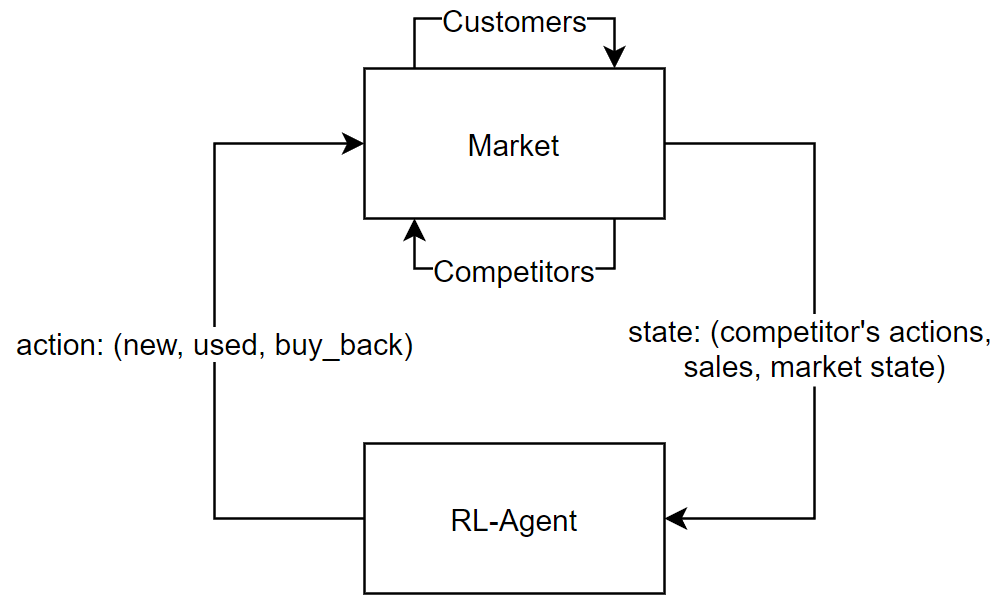
\includegraphics[height = 4 cm]{graphics/RL-Overview.png}\\[1 ex]
	\caption{The standard reinforcement-learning model in the context of our market.}
	\label{fig:IntroRLDiagram}
\end{figure}

Reinforcement-learning agents are trained through a process of trial-and-error. They interact with the market through an observable state
and an action which influences the following state. \Cref{fig:IntroRLDiagram} illustrates the RL-model in the context of our
market.\todo{Create a \emph{nicer} diagram with the three prices} The goal of the agent is to maximize the so-called reinforcement signal,
which in our case is the profit the agent made during the last cycle, since we want to train agents to maximize profits on real markets.
By observing which prices lead to which reinforcement signal, the agents get more profitable over the course of training.


\chapter{Related Work}
\section{Packaging discussion in the Python community}

\chapter{What makes a good agent?}
\section{Good agent = high profit, few outliers}
\section{Overview of market components}
\subsection{Focus on how agents make profit etc.}
\section{How realistic the market is}
\subsection{Restrictions for evaluation arising from this}

\chapter{Different approaches}
\section{During vs. After training}
\section{Tensorboard? (Not built by us)}
\section{Macro}
\subsection{Agent-monitoring}
\subsection{Live-monitoring}
\section{Micro}
\subsection{Exampleprinter}
\section{Static}
\subsection{Policyanalyzer}

\chapter{Our workflow}
\section{Training continuously saves models}
\subsection{Automatic monitoring at certain intervals}
\subsection{-> Can we discard agents prematurely due to results from this?}
\subsection{First analysis if available with finished training}

\section{Manual invocation of monitoring functionalities}
\subsection{When is this necessary/a good idea? Why?}

\chapter{Interpreting the results}
\section{Graphs and diagrams are available...}
\subsection{...comparing with other agents/models}
\subsection{...which hyperparameters influence the results in what ways?}
\subsection{...can we augment e.g. Grid-Search with our analysis?}
\subsection{-> Would need to make results "machine-readable" again}


%%%%%%%%%%%%%%%%%%%%%%%%%%%%%%%%%
%% End of adding your content. %%
%%%%%%%%%%%%%%%%%%%%%%%%%%%%%%%%%


% Add the following chapters not to the current ›part‹ but one level above instead.
\makeatletter
\def\toclevel@chapter{-1}
\def\toclevel@section{0}
\makeatother

\chapter{Conclusions \& Outlook}
% This is where you conclude your thesis.



% Following are the files and commands for the bibliography and the author’s publications.
\pagestyle{plain}

\renewcommand*{\bibfont}{\small}
\printbibheading
\addcontentsline{toc}{chapter}{Bibliography}
\printbibliography[heading = none]

\addchap{Declaration of Authorship}
I hereby declare that this thesis is my own unaided work. All direct or indirect sources used are acknowledged as references.\\[6 ex]

\begin{flushleft}
    Potsdam, \today
    \hspace*{2 em}
    \raisebox{-0.9\baselineskip}
    {
        \begin{tabular}{p{5 cm}}
            \hline
            \centering\footnotesize\printAuthor
        \end{tabular}
    }
\end{flushleft}


\end{document}